\documentclass[a4paper, 11pt, titlepage]{article}
\usepackage{ucs}
\usepackage[german,ngerman]{babel}
\usepackage{fontenc}
\usepackage[pdftex]{graphicx}
\usepackage{color}

\renewcommand*{\thesubsection}{\alph{subsection}.}

\begin{document}
\title{Datenbanken \\
Ausarbeitung \"Ubung 4}

\author{Jakob Schulz}

\date{30. Oktober 2023}

\maketitle{\thispagestyle{plain}}

\section{Aufgabe}

\subsection{}
Die Spalte c kann den Wert null enthalten. Dies verbietet das RDBMS, denn sonst könnte nur ein Wert null sein. Null steht jedoch für noch nicht vergebene Daten.
\subsection{}
\begin{verbatim}
create table t(c int not null);
alter table t add primary key(c)
\end{verbatim}
\section{Aufgabe}
\subsection{}
Es wird versucht den Prim"arschlüssel aus t1 zu l"oschen. Problem hierbei ist, dass bereits der Prm"arschl"ussel referenziert wird. (Fremdschl"ussel von von t2 verweist auf t1.)
\subsection{}
\begin{verbatim}
drop table if exists t1;
create table t1
(
id int primary key
);
insert into t1 values(4711);
drop table if exists t2;
create table t2
(
id int primary key,
c int references t1
);
insert into t2 values(0,4711);
delete from t2;
delete from t1; 
\end{verbatim}
\subsection{}
\begin{verbatim}
drop table t1;
create table t1(
id int primary key
);
insert into t1 values(4711);
drop table t2;
create table t2(
id int primary key,
c int references t1 on delete set null
);
insert into t2 values(0,4711);
delete from t1;

--> Hier fehlt der Zusatz "drop table if exists ...", 
     deshalb müsste zuerst Tabelle t2 gelöscht werden
\end{verbatim}
Durch den Zusatz: "`on delete set null"' k"onnen Datens"atze (trotz Referenz auf t1) von t1 gel"oscht werden. \\
Die Daten von t2, welche auf die gelöschten Daten verwiesen haben werden auf null gesetzt.

\subsection{}
\begin{verbatim}
drop table t1;
create table t1(
id int primary key
);
insert into t1 values(4711);
drop table t2;
create table t2(
id int primary key,
c int references t1 on delete cascade
);
insert into t2 values(0,4711);
delete from t1;
\end{verbatim}
Auswirkungen: "`on delete cascade"' bewirkt, dass die Datensätze aus t2, welche auf den zu l"oschenden Datensatz aus t1 verweisen, mitgel"oscht werden.

\subsection{}
\begin{verbatim}
delete from t1;
delete from t2;
create table t3(
id int primary key,
d int references t2 on delete cascade)

--> Hier fehlt der Zusatz "drop table if exists ...", 
     deshalb müsste zuerst Tabelle t2 gelöscht werden
\end{verbatim}

\subsection{}
\begin{verbatim}
alter table t1 add column c int
\end{verbatim}

\subsection{}
\begin{verbatim}
alter table t1 add foreign key(c) references t3
\end{verbatim}
\subsection{}
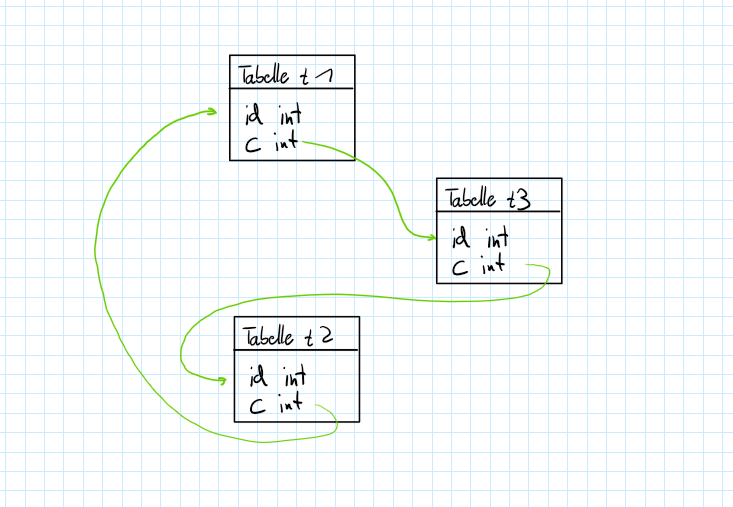
\includegraphics [width = 10cm]{Faustskizze_Teilaufgabe_h}\\
\subsection{}
Man kann nicht einfach einen Datensatz eingeben, denn man m"usste immer auf eine andere Tabelle referenzieren, welche jedoch noch keinen Datensatz besitzt. (Einzige Möglichkeit etwas einzuf"ugen: insert into t1 values(1, null)
\subsection{}
\begin{verbatim}
create table t1(
id int primary key,
c int
);
insert into t1 values(4711, 0);
create table t2(
id int primary key,
c int references t1 on delete cascade
);
insert into t2 values(3,4711);
create table t3(
id int primary key,
c int references t2 on delete cascade);
insert into t3 values(0,3);
alter table t1 add foreign key(c) references t3
\end{verbatim}
\subsection{}
delete from t3 $\Rightarrow$ Fehler weil delete on cascade fehlt
\subsection{Zusatz Informationen}
delete from "`tabelle"' $\Rightarrow$ Löscht Datensätze
\section{Aufgabe}
\subsection{}
\begin{verbatim}
alter table titanic add column embarked_id int;
\end{verbatim}
\subsection{}
\begin{verbatim}
alter table titanic add foreign key(embarked_id) 
references embarked;;
\end{verbatim}
\subsection{}
Die Spalte embarked\_id enth"alt keine Werte $\Rightarrow$ enth"alt null $\Rightarrow$ Werte sind noch nicht festgelegt
\begin{verbatim}
update titanic
set embarked_id = 2
where embarked = 'C';
update titanic
set embarked_id = 3
where embarked = 'Q';
update titanic
set embarked_id = 4
where embarked = 'S';
\end{verbatim}
\subsection{}
Die Spalte embarked ist in der Tabelle titanic "uberfl"ussig, weil es nun eine Tabelle gibt, welche mit referenizieler Integrität den richtigen Zustiegshafen jeder Person zuordnet.
\begin{verbatim}
alter table titanic drop column embarked
\end{verbatim}
\subsection{}
\begin{verbatim}
alter table embarked drop column ortkuerz;
\end{verbatim}
\subsection{}
\begin{verbatim}
alter table embarked add constraint ortsname_unique unique(ortsname);
\end{verbatim}
\subsection{}
\begin{verbatim}
Delete from embarked
where o_id = 1
\end{verbatim}
\end{document}